% Second-order dissociation of a Hubbard bound pair in a common spatially correlated lattice potential
% English journal draft v1 (target: J. Phys. A: Math. Theor.), compiled from the Chinese review copy v1.5.
% JPA accepts common LaTeX classes; 12 pt body text follows the current author guidance.
\documentclass[12pt,a4paper]{article}
\usepackage[T1]{fontenc}
\usepackage{lmodern}
\usepackage[margin=2.5cm]{geometry}
\usepackage{amsmath,amssymb,amsthm}
\usepackage{graphicx}
\usepackage{booktabs}
\usepackage{array}
\newcolumntype{L}[1]{>{\raggedright\arraybackslash}p{#1}}
\newcolumntype{C}[1]{>{\centering\arraybackslash}p{#1}}
\renewcommand{\arraystretch}{1.1}
\setlength{\emergencystretch}{2em}
\usepackage[font=small,labelfont=bf]{caption}
\captionsetup[table]{position=top,skip=6pt}
\usepackage{xcolor}
\usepackage[colorlinks=true,linkcolor=blue!50!black,citecolor=blue!50!black,urlcolor=blue!50!black]{hyperref}

\urlstyle{same}
\hypersetup{pdfauthor={JIN HANZHE},pdftitle={Second-order dissociation of a Hubbard bound pair in a common spatially correlated lattice potential}}

\newtheorem{proposition}{Proposition}
\newtheorem{corollary}{Corollary}
\newtheorem{lemma}{Lemma}
\theoremstyle{remark}
\newtheorem{remark}{Remark}

\newcommand{\Kd}{\mathcal{K}_d}
\newcommand{\wrap}{\operatorname{wrap}}
\newcommand{\sgn}{\operatorname{sgn}}
\newcommand{\sinc}{\operatorname{sinc}}
\newcommand{\E}{\mathbb{E}}
\newcommand{\Ustar}{U_{*}}
\providecommand{\eprint}[2][]{\href{https://arxiv.org/abs/#2}{arXiv:#2}}
\title{Second-order dissociation of a Hubbard bound pair\\ in a common spatially correlated lattice potential}
\author{JIN HANZHE\\[2pt]
\small Independent Researcher, Chongqing, China\\
\small Corresponding author: \href{mailto:jinhanzhe09@gmail.com}{jinhanzhe09@gmail.com}}
\date{}

\begin{document}
\maketitle

\begin{abstract}
We consider two bosons in the one-dimensional Bose--Hubbard model with hopping amplitude $J$ and constant on-site repulsion $U$, both subject to the same weak, static, stationary Gaussian lattice potential. For a repulsively bound pair of total quasimomentum $K$ we derive in closed form the second-order (golden-rule) kernel for transitions into the interacting two-particle scattering continuum at transferred momentum $q$. The kernel is strictly positive throughout the kinematically open region and vanishes as a square root at its edges. Its continuum factor coincides with that of the known dissociation rate under hopping modulation, while the static density coupling contributes a momentum-dependent form factor and a folded on-shell support. For flat high-pass disorder spectra the kernel gives an exact classification of when dissociation and elastic backscattering vanish at order $W^2$ in the disorder strength. For $\pi/2<|K|<\pi$ and $U<4J\sin(|K|/2)$, a critical interaction $\Ustar=4J\sqrt{-\cos K}$ separates pairs whose second-order dissociation can be removed by a finite spectral gap from those for which it cannot, and there is a window in which backscattering is closed while dissociation stays open. As the gap edge $q_0$ approaches the largest open transfer $q_c$, the coefficient vanishes as $\Delta^{3/2}$, $\Delta^{1/2}$ or $\Delta$, with $\Delta=q_c-q_0$, or tends to a nonzero plateau, depending on the geometry of the open region and on whether the pass-band height or the on-site variance is held fixed. Exact finite-ring simulations of the bound-band population reproduce the predicted enhancement and suppression for the two normalizations.
\end{abstract}

\noindent\textbf{Keywords:} Hubbard model, bound pairs, correlated disorder, Fermi golden rule, dissociation, scattering continuum

%======================================================================
\section{Introduction}
%======================================================================

At each total quasimomentum $K$, two particles on a lattice with on-site repulsion form a bound pair whose energy lies above the scattering continuum of the same momentum sector. If the repulsion is weak enough, this energy can still fall inside the continuum of another sector $K+q$; a static potential that supplies the momentum $q$ can then dissociate the pair without any change of energy. Repulsively bound pairs have been prepared with ultracold atoms in optical lattices~\cite{Winkler2006}, and the two-body problem of the Hubbard model is solved exactly, including the bound state and the interacting scattering states for every total quasimomentum~\cite{ValientePetrosyan2008}. When translation invariance is broken, the pair can scatter elastically into other bound states or dissociate. Dissociation has been analysed for periodic hopping modulation, where the golden-rule rate is known~\cite{Javanainen2010}, for a common localized trap~\cite{MaksimovKolovsky2014} and for random interaction strengths, which dissociate the pair at order $W^2$~\cite{Perrin2021}. The internal form factor of a pair moving in a common potential is also known~\cite{TurekJohn2003}, and for a common quasiperiodic potential an exact equation projected onto the contact site is available~\cite{DufourOrso2012}.

For correlated disorder, the power spectrum $S(q)$ of the potential determines which momentum transfers are available. This principle underlies selective transport in waveguides with correlated surface disorder~\cite{IzrailevMakarov2003,IzrailevMakarov2004}, the effective mobility edges of speckle potentials~\cite{Lugan2009,GurevichKenneth2009} and the hierarchy of localization lengths in high-pass (``stealthy'') lattice disorder~\cite{Vanoni2026}. For a composite particle the spectrum enters through an internal matrix element, and for dissociation the final states form a continuum whose weight depends on the interaction. Here we ask which momentum transfers dissociate a bound pair in a common static lattice potential at second order, with what weight, and when a spectral gap removes this channel.

Our main results are as follows. (i) We obtain the second-order dissociation kernel $\Kd(q)$ in closed form, equation~\eqref{eq:kernel}, and show that it is strictly positive on the whole open region $\Omega$. Its continuum factor $D/(D^2+U^2)$, and with it the square-root edge, already appears in the hopping-modulation rate of reference~\cite{Javanainen2010}; the static density coupling adds the form factor $B(q)^{-2}$ and a folded on-shell support. (ii) For any non-negative integrable spectrum, the $O(W^2)$ coefficient vanishes if and only if $S=0$ almost everywhere on $\Omega$. For flat high-pass spectra this gives a classification in the $(K,U)$ plane, with the critical interaction $\Ustar$ and a window that closes backscattering but not dissociation (figure~\ref{fig:classification}, table~\ref{tab:classification}). (iii) Near the largest open transfer $q_c$, the coefficient vanishes as $\Delta^{3/2}$, $\Delta^{1/2}$ or $\Delta$, or tends to a nonzero plateau, and the two common normalizations of high-pass disorder, fixed pass-band height and fixed on-site variance, can change the rate in opposite directions (figures~\ref{fig:classification} and~\ref{fig:endpoints}). (iv) Exact dynamics on finite rings, with the full clean bound band as observable, reproduce these opposite trends (section~\ref{sec:numerics}).

Throughout, ``closure'' means that the $W^2$ coefficient vanishes. The first nonvanishing higher order is set by the support of multiple momentum transfers and need not be $W^4$ (appendix~\ref{app:higher}). We do not consider finite-$W$ lifetimes, many-body doublon relaxation~\cite{Chudnovskiy2012} or bound states in the continuum created by isolated impurities~\cite{ZhangBraakKollar2012}.

%======================================================================
\section{Model, observable and normalization}\label{sec:model}
%======================================================================

We set the lattice constant and $\hbar$ to one and take $J>0$, $U>0$:
\begin{equation}\label{eq:H}
H=-J\sum_j\bigl(b_{j+1}^\dagger b_j+\mathrm{h.c.}\bigr)+\frac{U}{2}\sum_j n_j(n_j-1)+\sum_j w_j n_j .
\end{equation}
Both particles experience the same real, stationary, zero-mean Gaussian potential $w_j$ with covariance
\begin{equation}\label{eq:spectrum}
\E(w_jw_{j+r})=W^2\int_{-\pi}^{\pi}\frac{dq}{2\pi}\,S(q)\,e^{iqr},\qquad
S_H(q)=\mathbf{1}_{q_0<|q|<\pi},\qquad S_V(q)=\frac{S_H(q)}{1-q_0/\pi},
\end{equation}
where $S\in L^1([-\pi,\pi))$ is a non-negative even spectral density, defined up to sets of measure zero; spectra with Dirac components are not considered. Momenta are represented in $[-\pi,\pi)$ and $\wrap$ maps a real number to this interval. The two flat high-pass families with $0\le q_0<\pi$ keep either the pass-band height ($S_H$) or the on-site variance ($S_V$) fixed; only for $S_V$ is $W$ the ensemble standard deviation of $w_j$.

The initial state is the clean bound eigenstate with total quasimomentum $K$. The observable is the projector $P_B$ onto the entire clean bound band (all total momenta), and the loss is $L(T)=1-\E\langle P_B(T)\rangle$. Unlike the return probability or the double occupancy, $P_B$ is conserved by the clean dynamics~\cite{Boschi2014} and is insensitive to the fast oscillations of on-site observables~\cite{Bello2017}; it changes only through transitions into the continuum. At fixed ring size $N$ and time $T$ we write $L(T)=W^2\ell_N(T)+O(W^4)$ and define the second-order coefficient by the ordered limits
\begin{equation}\label{eq:c-def}
c=\lim_{T\to\infty}\frac{1}{T}\lim_{N\to\infty}\ell_N(T),\qquad \Gamma^{(2)}=W^2c .
\end{equation}
$\Gamma^{(2)}$ is the golden-rule rate, not the inverse lifetime at finite $W$.

The finite-ring construction behind~\eqref{eq:c-def} uses a bounded, piecewise-continuous representative of $S$, which covers both flat families at every fixed $q_0<\pi$, and allowed incoming momenta $K_N\to K$. For a general non-negative $L^1$ density we take the integral in~\eqref{eq:kernel} as the definition of $c$; since the kernel is bounded, this does not depend on the representative, and proposition~\ref{prop:closure} refers to this definition.

In first quantization the two-boson space is embedded isometrically in the symmetric part of $\ell^2(\mathbb{Z}_N^2)$, and in each total-momentum block the problem reduces to a relative coordinate $r$ with relative hopping $t_K=2J\cos(K/2)$ (appendix~\ref{app:P1}). On an even ring the gauge-transformed relative function is antiperiodic for odd momentum index, a point that matters for finite-size checks but not for the infinite-chain results below.

%======================================================================
\section{The dissociation kernel}\label{sec:kernel}
%======================================================================

Let $t_0=2J\cos(K/2)$ and $t\equiv t_q=2J\cos[(K+q)/2]$ be the incoming and outgoing relative hoppings. The incoming bound state is~\cite{ValientePetrosyan2008}
\begin{equation}\label{eq:bound}
E=\sqrt{U^2+4t_0^2},\qquad b_K(r)=C a^{|r|},\qquad a=-\frac{2t_0}{E+U},\qquad C^2=\frac{U}{E}.
\end{equation}
A momentum transfer $q$ from the common potential acts on the relative wave function as the source $s_q(r)=2Ca^{|r|}\cos(qr/2)$. The outgoing relative Hamiltonian $h(t)=-t(\mathcal{T}+\mathcal{T}^\dagger)+U|0\rangle\langle0|$, with $\mathcal{T}$ the relative translation, has the even, $\delta$-normalized scattering states
\begin{equation}\label{eq:scattering}
\phi_{p,t}(r)=\frac{D_p\cos(pr)+U\sgn(t)\sin(p|r|)}{\sqrt{\pi\,(D_p^2+U^2)}},\qquad D_p=2|t|\sin p,\qquad e_p=-2t\cos p,
\end{equation}
with each $p\in(0,\pi)$ counted once. Odd scattering states are orthogonal to the even source.

\begin{proposition}[Dissociation kernel]\label{prop:kernel}
Let $D(q)=\sqrt{4t_q^2-E^2}$ and $B(q)=1-4\cos^2(K/2)\,t_q^2/E^2$. On the open region $\Omega=\{q\in[-\pi,\pi):4t_q^2>E^2\}$,
\begin{equation}\label{eq:kernel}
\begin{aligned}
\Kd(q)&=2\pi\int_0^\pi dp\,|\langle\phi_{p,t_q}|s_q\rangle|^2\,\delta(E-e_p)
=\frac{8(U/E)^3\,D}{(D^2+U^2)\,B^2}>0,\\
c&=\int_{-\pi}^{\pi}\frac{dq}{2\pi}\,S(q)\,\Kd(q),
\end{aligned}
\end{equation}
and $\Kd=0$ outside $\Omega$. Moreover $B\ge U^2/E^2$, $\Kd$ is bounded for fixed $U>0$, and $\Kd\propto D$ as $D\to0$.
\end{proposition}

The proof (appendix~\ref{app:P3}) evaluates the overlap by summing geometric series and imposes the on-shell condition $\cos p=-E/(2t)$, under which the matrix element reduces to $F=(U/E)/B$ and $\Kd=8C^2DF^2/(D^2+U^2)$. The bound $B\ge U^2/E^2$ follows from $t_q^2\le4J^2$; it controls the denominator but is not a uniform lower bound on $\Kd$, which vanishes at the edges of $\Omega$. The $1/D$ singularity of the free density of states is cancelled by the interacting scattering states, so the edge behaviour cannot be estimated from the free continuum. Since $\Kd$ depends on $t_q$ only through $t_q^2$, it is invariant under $q\to q+2\pi$, as required: shifting $q$ by $2\pi$ changes the sign of $t$ and multiplies the source by $(-1)^r$, and both are generated by the same unitary.

\begin{remark}[Comparison with modulation spectroscopy]
Javanainen, Odong and Sanders~\cite{Javanainen2010} obtained the golden-rule dissociation rate of the same dimer under a periodic modulation of the hopping with depth $\Lambda$. In the present units their result can be written as $\Gamma_{\rm mod}=(\Lambda^2U^3/2E_b)\,D_0/(U^2+D_0^2)$, where $D_0=\sqrt{\Omega_P^2-e^2}$ and the outgoing relative energy $e$ is selected by the drive frequency (appendix~\ref{app:prior}). The factor $D/(U^2+D^2)$, and with it the square-root edge, is thus a property of the interacting even continuum. The static common potential differs in three respects: it changes the total momentum $K\to K+q$ at fixed energy; the overlap of the source $2Ca^{|r|}\cos(qr/2)$ with the scattering state produces the form factor $B(q)^{-2}$; and the support $\Omega$ is fixed by static energy conservation and lattice folding.
\end{remark}

\begin{remark}[Role of positivity]
The closure criterion of section~\ref{sec:closure} requires only $\Kd>0$ almost everywhere on $\Omega$. Real analyticity gives this on every connected component of $\Omega$ on which $\Kd$ does not vanish identically, but it cannot exclude identically vanishing components, such as a selection rule might produce. The explicit form~\eqref{eq:kernel} rules them out, together with isolated dark points inside $\Omega$.
\end{remark}

%======================================================================
\section{Second-order closure and classification}\label{sec:closure}
%======================================================================

\begin{proposition}[Closure criterion]\label{prop:closure}
For every non-negative $S\in L^1([-\pi,\pi))$, with $c$ defined by the integral in~\eqref{eq:kernel},
\begin{equation}\label{eq:closure}
c=0\quad\Longleftrightarrow\quad S(q)=0\ \text{ for almost every } q\in\Omega .
\end{equation}
\end{proposition}

This follows from proposition~\ref{prop:kernel} and the fact that a non-negative integral vanishes only if the integrand vanishes almost everywhere (appendix~\ref{app:P4}). Supports may touch at endpoints, and null sets play no role.

\paragraph{Kinematics.} If $E\ge4J$, $\Omega$ is empty and $c=0$. If $E<4J$, let $k=|K|$ and $Q=2\arccos(E/4J)$; then $0<Q<k$ and $\Omega=\{q:|\wrap(K+q)|<Q\}$. The supremum of $|q|$ on $\Omega$ is
\begin{equation}\label{eq:qc}
q_c=\min(\pi,\,k+Q).
\end{equation}

\begin{corollary}[Flat high-pass spectra]\label{cor:highpass}
For $E<4J$ and a nonempty flat high-pass spectrum ($S_H$ or $S_V$), $c=0$ if and only if $q_c<\pi$ and $q_0\ge q_c$. For $\pi/2<k<\pi$ the continuum is reachable when $U<U_E=4J\sin(k/2)$, and
\begin{equation}\label{eq:Ustar}
k+Q=\pi\quad\Longleftrightarrow\quad U=\Ustar,\qquad \Ustar=4J\sqrt{-\cos k}.
\end{equation}
For $U\le\Ustar$ one has $q_c=\pi$ and no $q_0<\pi$ removes the $W^2$ coefficient; for $\Ustar<U<U_E$ a finite gap $q_0\ge q_c$ does. For $k\le\pi/2$ every pair with $E<4J$ has $q_c<\pi$.
\end{corollary}

Physically, at $U=\Ustar$ the bound state at $K$ is degenerate with the upper edge of the two-particle continuum at $K+\pi$. Every flat high-pass spectrum contains transfers arbitrarily close to $\pi$; at $U=\Ustar$ one side of this point lies in $\Omega$ and at $U<\Ustar$ both sides do, so no nonempty flat high-pass spectrum removes dissociation at second order.

\paragraph{Elastic backscattering.} For $0<k<\pi$ the bound pair can also scatter elastically to $-K$, with momentum transfer $q_B=|\wrap(2K)|$, group velocity $|v_B|=4J^2|\sin K|/E$ and overlap
\begin{equation}\label{eq:FB}
F_B=\frac{2(1-a^2)^2}{1-2a^2\cos K+a^4}>0 .
\end{equation}
Away from spectral discontinuities the backscattering coefficient is $F_B^2S(q_B)/|v_B|$. For a hard high-pass edge, strict closure requires $q_0>q_B$: at $q_0=q_B$ (with $0<q_B<\pi$) the finite-time kernel $T\sinc^2(T\,\Delta E/2)$ is even about the resonance and assigns half of the pass-band weight to each side of the step, so in the ordered limit~\eqref{eq:c-def} the backscattering coefficient takes half of its pass-band value. Redefining $S$ at a single point does not change this. At the dissociation edge the situation is different: the coefficient is an integral over an interval on which $\Kd\to0$, so $q_0=q_c$ closes dissociation.

\paragraph{Windows.} Backscattering is closed while dissociation remains open for $q_B<q_0<q_c$. For $0<k<\pi/2$, $q_c<q_B=2k$ and no such window exists; for $k=\pi/2$, $q_B=\pi$ and no nonempty high-pass spectrum closes backscattering. For $\pi/2<k<2\pi/3$ the window exists if and only if
\begin{equation}\label{eq:window}
U<4J\sqrt{-\sin(2k)\sin k},
\end{equation}
and for $2\pi/3\le k<\pi$ it exists for every pair with $E<4J$. Both channels are closed at second order for $q_0>q_B$ and $q_0\ge q_c$, which requires $q_B<\pi$ and $q_c<\pi$ (appendix~\ref{app:P5}). Table~\ref{tab:classification} summarizes the classification; figure~\ref{fig:classification} shows it together with $c(q_0)$ for both normalizations.

\begin{table}[t]
\centering
\caption{Second-order classification for flat high-pass spectra ($0<k<\pi$). ``Closed'' means that the $W^2$ coefficient vanishes.}
\label{tab:classification}
\begin{tabular}{@{}L{0.27\textwidth}L{0.27\textwidth}L{0.40\textwidth}@{}}
\toprule
Condition & Dissociation & Backscattering \\
\midrule
$E\ge4J$ & closed ($c=0$) & closed iff $q_0>q_B$; half weight at $q_0=q_B$\\
$E<4J$, $q_c<\pi$ & closed iff $q_0\ge q_c$ & as above\\
$E<4J$, $q_c=\pi$ ($U\le\Ustar$) & open for every $q_0<\pi$ & as above\\
$q_B<q_0<q_c$ & open & closed\\
\bottomrule
\end{tabular}
\end{table}

\begin{figure}[t]
\centering
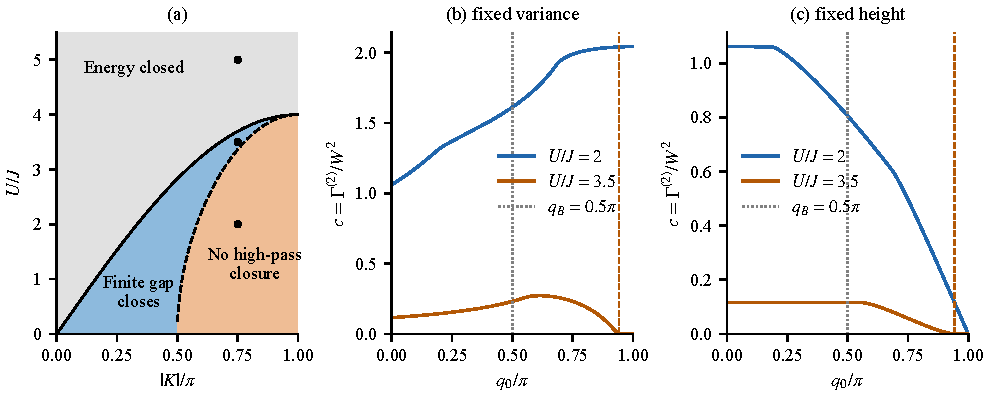
\includegraphics[width=\textwidth]{figures/fig1_classification.pdf}
\caption{(a) Second-order dissociation in the $(|K|,U)$ plane for $J=1$. Grey: $E\ge4J$, no on-shell continuum. Blue: $q_c<\pi$, so a flat high-pass spectrum with $q_0\ge q_c$ removes the $W^2$ coefficient. Orange: $U\le\Ustar$, $q_c=\pi$, no nonempty high-pass spectrum does. Solid line: $U_E=4J\sin(k/2)$; dashed line: $\Ustar=4J\sqrt{-\cos k}$. Dots mark $K=0.75\pi$ with $U=2$, $3.5$ and $5$, the parameters used in section~\ref{sec:numerics}. (b), (c) Coefficient $c=\Gamma^{(2)}/W^2$ versus $q_0$ at $K=0.75\pi$ for fixed on-site variance (b) and fixed pass-band height (c). Dotted line: $q_B=0.5\pi$, backscattering is closed for $q_0>q_B$. Dashed line: $q_c=0.9417\pi$ for $U=3.5$; for $U=2$, $q_c=\pi$.}
\label{fig:classification}
\end{figure}

\paragraph{Beyond second order.} With $n$ insertions of the potential, the total momentum transfer lies in the $n$-fold sum of the pass band, which need not reach $\Omega$ for $n=2$. At $K=0.75\pi$, $U=3.5$ and $q_0=0.97\pi$, for example, one and two transfers miss $\Omega$ and three are the first to overlap it with positive measure, so an on-shell dissociation amplitude is first kinematically allowed at order $W^3$ (appendix~\ref{app:higher}). We have not computed this amplitude.

%======================================================================
\section{Behaviour near the closure edge}\label{sec:endpoints}
%======================================================================

We fix $J$, $K$ and $U>0$ with $Q>0$, define $c_H(\Delta)$ and $c_V(\Delta)$ by~\eqref{eq:c-def} for each $\Delta=q_c-q_0>0$, and only then let $\Delta\downarrow0$.

\begin{proposition}[Endpoint asymptotics]\label{prop:endpoints}
(a) Interior threshold, $q_c=k+Q<\pi$: near the edge $\Kd\simeq A\sqrt{x}$, with $x$ the distance from the edge inside $\Omega$ and
\begin{equation}\label{eq:A}
A=\frac{8U\sqrt{8J^2\sin Q}}{E^3\sin^4(k/2)},\qquad
c_H\sim\frac{A\,\Delta^{3/2}}{3\pi},\qquad c_V\sim\frac{A\,\Delta^{3/2}}{3\pi\,(1-q_c/\pi)} .
\end{equation}
(b) Critical case, $\pi/2<k<\pi$ and $U=\Ustar$ ($q_c=\pi$): $c_H\sim A\Delta^{3/2}/(3\pi)$ but $c_V\sim A\sqrt{\Delta}/3$.\\
(c) Wrapped case, $\pi/2<k<\pi$ and $U<\Ustar$: $c_H\sim\Kd(\pi)\,\Delta/\pi$ and $c_V\to\Kd(\pi)>0$.
\end{proposition}

At the edge $t^2=E^2/4$, $B=\sin^2(k/2)$ and $D^2=8J^2\sin Q\,x+O(x^2)$, which gives the square-root law and, after integration over an interval of length $\Delta$, the $3/2$ law. In the critical case $\pm\pi$ is a single point of the ring with only one side inside $\Omega$, while the fixed-variance normalization divides by $1-q_0/\pi=\Delta/\pi$; this lowers the exponent to $1/2$. For $U<\Ustar$ the point $\pi$ lies inside $\Omega$, both sides of the pass band contribute, and the fixed-variance coefficient tends to the plateau $\Kd(\pi)$. The plateau has a simple origin. As $\Delta\to0$ the fixed-variance potential converges in finite-dimensional distributions to a staggered field with a single random amplitude (appendix~\ref{app:P6}), whose momentum transfer $\pi$ couples the pair at $K$ to the open continuum at $K+\pi$; the limiting field, with its singular spectrum, is not itself in the class of section~\ref{sec:model}. The exponents follow from the square-root edge and the measure; the kernel supplies the coefficient $A$ and the difference between the two normalizations (figure~\ref{fig:endpoints}).

\begin{figure}[t]
\centering
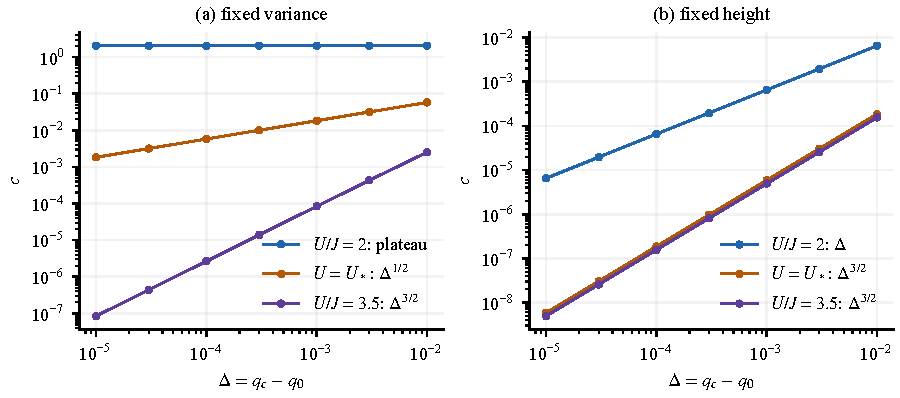
\includegraphics[width=0.92\textwidth]{figures/fig2_endpoints.pdf}
\caption{Second-order coefficient as $q_0\to q_c$ at $K=0.75\pi$, $\Delta=q_c-q_0$, evaluated from equation~\eqref{eq:kernel}. (a) Fixed on-site variance: plateau for $U=2<\Ustar$, $\Delta^{1/2}$ at $U=\Ustar$, $\Delta^{3/2}$ for $U=3.5$ (interior threshold). (b) Fixed pass-band height: $\Delta$ for $U=2$, $\Delta^{3/2}$ for $U=\Ustar$ and $U=3.5$.}
\label{fig:endpoints}
\end{figure}

\paragraph{Special limits.} For $K=0$, $E>4J$ and $c=0$. At $K=\pi$ the bound state is localized on the relative origin, $E=U$, and $\Kd=8D/(D^2+U^2)$; for $U<4J$ one has $q_c=\pi$, and since the group velocity vanishes the backscattering formula does not apply. At $E=4J$ the linear coefficient vanishes. If $S$ has a finite, nonzero local limit at $q=-K$, the joint spectral weight near the top of the continuum vanishes linearly in the energy offset and the second-order response can contain $\log T$; for other integrable spectra the threshold behaviour depends on the local spectral weight. A strict energy gap guarantees a bounded second-order virtual admixture. As $U\to0$ at fixed $0<k<\pi$, $\Kd$ develops a peak of width $O(U)$ and height $O(1/U)$ near $K+q=0$, and for $S$ continuous at $q=-K$
\begin{equation}\label{eq:smallU}
\lim_{U\downarrow0}c=\frac{S(K)}{J\sin(k/2)} ;
\end{equation}
here $U\to0$ is taken after $W\to0$, so the result does not describe a loosely bound pair at finite $W$ (appendix~\ref{app:P7}).

\paragraph{Finite disorder.} These asymptotics are taken after $W\to0$. At finite $W$ they require the detuning scale $g\simeq2J\sin(Q/2)\,\Delta$ to exceed the relative energy shifts of the bound state and of the continuum edge, the spectral broadening and the resolution $1/T$, and the remainder to stay small compared with $W^2c$. We do not derive such bounds here. Since the height of $S_V$ grows as $1/\Delta$, a $\Delta$-independent criterion such as $\Delta\gg CW^2$ cannot be assumed.

%======================================================================
\section{Numerical illustration}\label{sec:numerics}
%======================================================================

For all numerical results we use $J=1$, with energies in units of $J$ and times in units of $J^{-1}$. We simulated the exact dynamics of two bosons on rings of $N=128$ and $256$ sites in the symmetric $N^2$ representation, starting from the clean bound state at $K=0.75\pi$ and recording the clean bound-band population $P_B(T)$ (appendix~\ref{app:numerics}). Random potentials were generated by Fourier filtering of white Gaussian noise; the fixed-variance family was normalized by the actual number of allowed modes, without per-sample renormalization. The protocol, including the observable, the fitting window $T=12$--$24$ for $U=2$ (linear fit with intercept), the seeds and the pairing of spectral families through common raw noise, was fixed before the confirmatory runs.

\begin{table}[t]
\centering
\caption{Frozen primary result: $K=0.75\pi$, $U=2$, $N=256$, $W=0.04$, 32 paired seeds. Fitted slope of $L(T)$ over $T=12$--$24$, divided by $W^2$, with Student 95\% intervals (sampling uncertainty).}
\label{tab:numerics}
\begin{tabular}{@{}lccc@{}}
\toprule
Spectrum & $c$ (infinite chain) & Slope$/W^2$ & 95\% interval\\
\midrule
No gap & 1.061 & 1.031 & [0.991, 1.070]\\
$q_0=0.8\pi$, fixed variance & 2.013 & 1.832 & [1.699, 1.964]\\
$q_0=0.8\pi$, fixed height & 0.4027 & 0.3841 & [0.3551, 0.4132]\\
\bottomrule
\end{tabular}
\end{table}

Table~\ref{tab:numerics} shows the primary comparison. Relative to the ungapped spectrum, the paired ratios of mean slopes are $1.777$ $[1.691,1.858]$ for fixed variance and $0.373$ $[0.354,0.391]$ for fixed height (paired bootstrap, ratio of means), against $1.897$ and $0.379$ from equation~\eqref{eq:kernel}. The two normalizations thus move the dissociation rate in opposite directions, as predicted. The fixed-variance slope lies $9.0\%$ below $c$, outside its sampling interval.

A post hoc analysis of the saved trajectories (appendix~\ref{app:posthoc}) breaks this offset down as follows. The infinite-chain second-order response, fitted over the same seven time points, reproduces $c$ to better than $0.01\%$ for all three spectra, so the window itself causes no appreciable bias at second order on the infinite chain. For the same 32 noise realizations the finite-ring second-order prediction gives $\bar p/c=0.970$ (95\% interval $[0.898,1.039]$), compatible with $c$. The remaining factor, actual over predicted slope $0.938$, is reproduced to within $0.6\%$ by a parameter-free exponential surrogate that accounts for depletion of $P_B$ within the window, and it approaches one as $W$ decreases ($0.984$ at $W=0.02$). Changing $N$ from 128 to 256 or shifting the window changes the slopes by less than $2.5\%$ and leaves the direction of both effects unchanged.

Close to the closure edge ($U=3.5$, $q_0\ge0.9\pi$) finite-time recurrences prevent a stable estimate of an asymptotic rate; some fits even give negative slopes, which reflect recurrences rather than decay. At $U=5$, where $E>4J$, the sudden switch-on of the potential still produces a small virtual admixture outside the clean bound band. Thus $c=0$ implies neither $P_B(T)=1$ nor all-order stability.

\paragraph{Research workflow and AI use.}
Generative AI was used extensively in developing the analytic derivations, implementing and running numerical calculations, analysing the results, checking the literature and preparing the manuscript. The model identifiers and their respective roles are specified in the AI disclosure below. The research checks included state normalization, exchange symmetry, momentum folding, continuum endpoints, special limits and comparisons between scattering-state and resolvent calculations (appendices~\ref{app:proofs} and~\ref{app:checks}). The human author participated substantially in interpreting the results, verifying the principal conclusions and critically reviewing the manuscript. The Zenodo archive~\cite{JinZenodo2026} provides the executable code, saved observations, configurations and validation records, together with a description of the AI workflow; rerunning these calculations does not require access to the generative models.

%======================================================================
\section{Conclusions}\label{sec:conclusions}
%======================================================================

For a Hubbard bound pair in a common static lattice potential we have obtained the second-order dissociation kernel in closed form and shown that it is positive on the entire open region. Combined with the folded kinematics, it gives an exact criterion for when a spectral gap removes the $W^2$ dissociation coefficient, the critical interaction $\Ustar$ at and below which no high-pass spectrum does, the window in which backscattering is closed but dissociation open, and the endpoint coefficients for the two common normalizations of high-pass disorder. The half weight of elastic backscattering at a hard spectral step and the vanishing weight at the dissociation edge arise from different limits.

Several questions remain open: the order at which dissociation first appears beyond the second-order closure boundary, finite-$W$ corrections to the threshold, and the long-time fate of the pair. The closed-form kernel provides an analytic benchmark for such studies and for designing correlated potentials that act differently on the elastic and inelastic channels of a composite particle.

\section*{Data availability statement}
The data and code supporting the findings of this study are openly available in Zenodo at \url{https://doi.org/10.5281/zenodo.23390681}~\cite{JinZenodo2026}. The archive contains 752 confirmatory and 48 auxiliary observable trajectories, the corresponding seeds and configurations, saved second-order predictions, simulation and analysis code, figure data, validation records and instructions mapping the reported results to the files and commands needed to reproduce them.

\section*{Acknowledgements}

\paragraph{Funding.}
This research received no specific grant from any funding agency in the public, commercial or not-for-profit sectors.

\paragraph{Competing interests.}
The author declares no competing interests.

\paragraph{Author contributions.}
JIN HANZHE contributed substantially to the interpretation of the results, verification of the principal conclusions and critical review of the manuscript, approved the final version and accepts responsibility for the accuracy and integrity of the work.

\paragraph{AI disclosure.}
The \texttt{gpt-6-pro} model generated the initial research idea, performed the principal scientific review and participated in the final pre-submission review. The \texttt{gpt-6-astra-max} model carried out the main research work, and \texttt{opus5.5} assisted with review and drafted the manuscript. The final pre-submission review was carried out by \texttt{gpt-6-pro} and JIN HANZHE. The human author's verification and critical review covered the interpretation of the results and the principal conclusions, as described above; the author approved the manuscript and takes responsibility for its content. AI use in the research workflow and the accompanying validation materials are described in section~\ref{sec:numerics}.

%======================================================================
\appendix
%======================================================================

\section{Proofs}\label{app:proofs}

\subsection{Two-boson space and relative coordinate}\label{app:P1}

On a ring of $N$ sites the normalized Fock basis consists of $b_x^\dagger b_y^\dagger|0\rangle$ ($x<y$) and $(b_x^\dagger)^2|0\rangle/\sqrt2$. With Fock coefficients $F_{xy}$, the symmetric first-quantized amplitudes $\Psi_{xx}=F_{xx}$, $\Psi_{xy}=\Psi_{yx}=F_{xy}/\sqrt2$ satisfy $\sum_{x,y}|\Psi_{xy}|^2=\sum_{x\le y}|F_{xy}|^2$ and
\begin{equation}
(H\Psi)_{xy}=-J(\Psi_{x+1,y}+\Psi_{x-1,y}+\Psi_{x,y+1}+\Psi_{x,y-1})+(U\delta_{xy}+w_x+w_y)\Psi_{xy}.
\end{equation}
The map is an isometry and generates the $\sqrt2$ factors of on-site hopping automatically~\cite{ValientePetrosyan2008}. For $K=2\pi m/N$ set $\Psi(x,x+r)=N^{-1/2}e^{iKx}b_K(r)$. The hopping terms give $H_{r+1,r}=-J(1+e^{iK})$, and exchange symmetry requires $b_K(r)=e^{iKr}b_K(-r)$, $b_K(r+N)=b_K(r)$. With $b_K(r)=e^{iKr/2}u_K(r)$,
\begin{equation}
u_K(r)=u_K(-r),\qquad u_K(r+N)=(-1)^m u_K(r),\qquad h(t_K)=-t_K(\mathcal{T}+\mathcal{T}^\dagger)+U|0\rangle\langle0| .
\end{equation}
For even $N$ the exchange-fixed point $r=N/2$ must vanish when $m$ is odd, so the block dimensions are $N/2+1$ ($m$ even) and $N/2$ ($m$ odd); for odd $N$ every block has dimension $(N+1)/2$. In both cases the total is $N(N+1)/2$. Treating all blocks as periodic even chains gives wrong dimensions and wrong boundary spectra.

\subsection{Bound state, source, continuum normalization and folding}\label{app:P2}

The recursions at $r\neq0$ and $r=0$ give $E=-t_0(a+a^{-1})$ and $U=t_0(a-a^{-1})$, hence~\eqref{eq:bound}; $|a|<1$ and $\sum_r a^{2|r|}=(1+a^2)/(1-a^2)$ give $C^2=(1-a^2)/(1+a^2)=U/E$. For $t_0=0$ ($K=\pi$) the solution is $E=U$, $b=\delta_{r0}$.

With $w_q=N^{-1}\sum_jw_je^{-iqj}$, the common potential $w_x+w_y$ maps $|K,r\rangle$ to $|K+q,r\rangle$ with the factor $1+e^{iqr}$; removing the outgoing gauge phase $e^{i(K+q)r/2}$ leaves $s_q(r)$. Because both particles couple to the same field, their contributions add in amplitude rather than in power.

For $r\neq0$ the scattering recursion gives $e_p$; the condition at $r=0$ gives the even wave $\cos(pr)+[U/(2t\sin p)]\sin(p|r|)$~\cite{ValientePetrosyan2008}. On the full integer chain $\sum_r\cos(pr)\cos(p'r)$ has $\delta$-part $\pi\delta(p-p')$, and the phase-shifted asymptotic cosine has the same coefficient; dividing by $\sqrt\pi$ and by the asymptotic amplitude $\sqrt{1+(U/D_p)^2}$ gives~\eqref{eq:scattering}. A stronger check of the absolute normalization is the completeness relation of the even sector,
\begin{equation}\label{eq:completeness}
\int_0^\pi dp\,\phi_{p,t}(r)\phi_{p,t}(r')+b_t(r)b_t(r')=\frac{\delta_{r,r'}+\delta_{r,-r'}}{2},
\end{equation}
where $b_t$ is the normalized bound state of $h(t)$; it also follows from the spectral decomposition of the rank-one perturbation $U|0\rangle\langle0|$, and it detects any common missing factor of $2$ or $\pi$.

\emph{Folding.} With $A|r\rangle=(-1)^r|r\rangle$ one has $h(-t)=Ah(t)A$. Under $q\to q+2\pi$, $t\to-t$ and $s_q\to As_q$, so $\langle s|\delta(E-h)|s\rangle$ is unchanged. Changing the sign of $t$ without transforming the source gives the wrong overlap.

\subsection{Proof of proposition~\ref{prop:kernel}}\label{app:P3}

\emph{Overall factor.} For the bounded, piecewise-continuous representative specified in section~\ref{sec:model}, define ring modes $q_m=2\pi m/N$ and $\E|w_{q_m}|^2=W^2S(q_m)/N$. The momentum sums converge to the corresponding integrals, with $N^{-1}\sum_m\to\int dq/(2\pi)$ and $K_N\to K$; finite assignments at the jumps do not change this limit. For the numerical flat masks the stated finite-mode normalization has the same limit at fixed $q_0<\pi$. The golden rule with the measure of appendix~\ref{app:P2} gives the first expression in~\eqref{eq:kernel}: the factor $\pi$ comes from the $p$-normalization, $D=|de_p/dp|$ from the energy $\delta$-function, and $1/2\pi$ from the $q$-measure.

\emph{Overlap.} Let $\theta=q/2$ and
\begin{equation}
R=\sum_{\sigma=\pm1}\frac{a\,e^{i(p+\sigma\theta)}}{1-a\,e^{i(p+\sigma\theta)}},\qquad F=1+\Re R+\frac{U}{2t\sin p}\Im R .
\end{equation}
Summing the geometric series gives $\langle\phi_{p,t}|s_q\rangle=2CD_pF/[\sqrt\pi\sqrt{D_p^2+U^2}]$, hence on shell $\Kd=8C^2DF^2/(D^2+U^2)$. With $d_\pm=1-2a\cos(p\pm\theta)+a^2$,
\begin{equation}
1+\Re R=\frac{(1-a^2)(1+a^2-2a\cos p\cos\theta)}{d_+d_-},\qquad
\Im R=\frac{2a\sin p\,[(1+a^2)\cos\theta-2a\cos p]}{d_+d_-}.
\end{equation}
Using $aU=-t_0(1-a^2)$ and, on shell, $2a\cos p=t_0(1+a^2)/t$,
\begin{equation}
F=\frac{(1-a^2)(1+a^2)(t^2+t_0^2-2tt_0\cos\theta)}{t^2d_+d_-}.
\end{equation}
Two identities complete the reduction. Expanding $t=2J\cos(K/2+\theta)$ gives $t^2+t_0^2-2tt_0\cos\theta=4J^2\sin^2\theta$; expanding $d_+d_-$ and inserting $\cos p=-E/(2t)$ and $E=-t_0(1+a^2)/a$ gives $t^2d_+d_-=4\sin^2\theta\,[J^2(1+a^2)^2-a^2t^2]$. Hence
\begin{equation}
F=\frac{(1-a^2)/(1+a^2)}{1-a^2t^2/[J^2(1+a^2)^2]}=\frac{U/E}{B},
\end{equation}
using $a^2/(1+a^2)^2=t_0^2/E^2$. The cancellation of $\sin^2\theta$ is legitimate because $q\equiv0$ is never on shell ($E^2=U^2+4t_0^2>4t_0^2$), and $t\neq0$ on shell. For $K=\pi$, $a=0$, $R=0$ and $F=1$, consistent with the formula. Finally $t^2\le4J^2$ gives $B\ge1-16J^2\cos^2(K/2)/E^2=U^2/E^2>0$. \qed

\emph{Independent representation.} With $z=E+i0$, $g_r=\lambda^{|r|}/(iD)$ and $\lambda=(-E+iD)/(2t)$ the free relative Green function, $G=G_0+UG_0|0\rangle\langle0|G_0/(1-Ug_0)$ and $\Kd=-2\Im\langle s|G|s\rangle$. This representation does not use the geometric-series reduction and is used for the numerical checks of appendix~\ref{app:checks}.

\subsection{Proof of proposition~\ref{prop:closure} and corollary~\ref{cor:highpass}}\label{app:P4}

For fixed $U>0$, $S\Kd$ is non-negative and integrable. If its integral vanishes, each set $A_n=\{q:S\Kd\ge1/n\}$ has measure zero, since otherwise $c\ge|A_n|/(2\pi n)$; hence $S\Kd=0$ almost everywhere, and $\Kd>0$ on $\Omega$ gives $S=0$ almost everywhere on $\Omega$. The converse is immediate. The same argument holds if $\Kd>0$ only almost everywhere on $\Omega$.

The top of the outgoing continuum is $4J|\cos[(K+q)/2]|$, so $\Omega$ coincides with $D^2>0$. Since $U>0$ implies $E>4J\cos(k/2)$, we have $Q<k$. Take $K=k>0$. If $k+Q<\pi$, $\Omega=(-k-Q,-k+Q)$; if $k+Q>\pi$, $\Omega=(-\pi,-k+Q)\cup(2\pi-k-Q,\pi)$; $K<0$ follows by reflection. The supremum of $|q|$ on $\Omega$ is $q_c$. A high-pass band overlaps $\Omega$ with positive measure unless $q_c<\pi$ and $q_0\ge q_c$; at $q_0=q_c$ the contact is a single point, so $c=0$. For $\pi/2<k<\pi$, the condition $E<4J$ is $U<U_E$, and $Q\ge\pi-k$ is equivalent to $E\le4J\sin(k/2)$, i.e.\ $U^2\le-16J^2\cos k$, which gives~\eqref{eq:Ustar}. For $k\le\pi/2$, $Q<k$ gives $k+Q<\pi$. \qed

\subsection{Backscattering}\label{app:P5}

Elastic final bound states satisfy $K'=\pm K$ mod $2\pi$; $q=0$ is the forward term. The bound-state overlap is $2CC'\sum_r(aa')^{|r|}\cos(qr/2)$. For $K'=-K+2\pi\ell$ one has $a'=(-1)^\ell a$ and $\cos(q/2)=(-1)^\ell\cos K$, and summation gives~\eqref{eq:FB}, which does not vanish for $0<k<\pi$. The group velocity follows from $E_b(K)=\sqrt{U^2+16J^2\cos^2(K/2)}$. Near the backscattering root the second-order probability per unit time is
\begin{equation}
\int\frac{dq}{2\pi}S(q)|F(q)|^2\,T\sinc^2\!\left(\frac{T[E_b(K+q)-E]}{2}\right),\qquad\sinc x=\frac{\sin x}{x}.
\end{equation}
The substitution $x=Tv_B(q-q_{\rm root})/2$ turns the kernel into an even nascent $\delta$-function; a continuous $S$ receives full weight and a step receives one half. Removing exactly one resonant Fourier mode on a finite ring and then taking $T\to\infty$ is a different limit.

For the windows: if $0<k<\pi/2$, $q_c=k+Q<2k=q_B$. If $\pi/2<k<2\pi/3$, $q_B=2\pi-2k$ and $q_B<q_c$ requires $Q>2\pi-3k$, i.e.\ $E<-4J\cos(3k/2)$; squaring and using $\cos^2(3k/2)-\cos^2(k/2)=-\sin(2k)\sin k$ gives~\eqref{eq:window}. If $2\pi/3\le k<\pi$, $q_B\le k<q_c$. \qed

\subsection{Proof of proposition~\ref{prop:endpoints}}\label{app:P6}

For $K>0$ and $q_c=k+Q<\pi$ the pass band retains only $q=-q_c+x$ with $0<x<\Delta$. At the edge $t^2=E^2/4$, $B=\sin^2(k/2)$, and
\begin{equation}
D^2=8J^2\sin Q\,x+O(x^2),\qquad \Kd=A\sqrt{x}+O(x^{3/2}).
\end{equation}
Integrating and dividing by $2\pi$ gives $c_H$; $c_V$ carries the extra factor $(1-q_0/\pi)^{-1}$, whose limit is finite. In the critical case $k+Q=\pi$, $\pm\pi$ is one point of the ring with only one side in $\Omega$, so no factor of two arises, and the normalization denominator is $\Delta/\pi$. For $U<\Ustar$ both sides of $\pm\pi$ lie in $\Omega$, the total length is $2\Delta$, and folding invariance gives equal limits $\Kd(\pi)$ on both sides. \qed

For the narrow-band interpretation, write $q_0=\pi-\Delta$. At every integer separation $r$ the fixed-variance covariance is
\begin{equation}\label{eq:staggered-limit}
\frac{\E(w_jw_{j+r})}{W^2}=(-1)^r\sinc(r\Delta)\longrightarrow(-1)^r.
\end{equation}
The finite-dimensional distributions therefore converge to those of $w_j=WX(-1)^j$, with one real standard Gaussian variable $X$. The spectral measures $S_V(q)\,dq/(2\pi)$ converge weakly to a unit point mass at $q=\pi$ on the momentum circle. Continuity of $\Kd$ at that point gives $c_V\to\Kd(\pi)$. The limiting periodic field has a singular spectral measure and lies outside the class of section~\ref{sec:model}; the statement concerns only the limit of $c_V$, taken after the ordered limits~\eqref{eq:c-def}.

\subsection{Special limits}\label{app:P7}

\emph{$K=\pi$.} Then $b=\delta_{r0}$, $E=U$, $\Kd=8D/(D^2+U^2)$ for $D^2>0$, and $\Ustar=U_E=4J$, so the open critical line of proposition~\ref{prop:endpoints} does not exist.

\emph{$E\to4J$.} Proposition~\ref{prop:endpoints} requires fixed $Q>0$; as $Q\to0$, $A\to0$ and the expansion is not uniform. Near the top of the total continuum, $4J-e\simeq JK'^2/2+2J(\pi-p)^2$, and the squared source overlap vanishes as $(\pi-p)^2$. If $S$ has a finite nonzero local limit at $q=-K$, the two-dimensional integral gives a joint spectral weight $\rho(\varepsilon)\propto\varepsilon$, hence a possible $\log T$ term in the second-order response at $E=4J$. A flat spectral step with a finite nonzero one-sided value changes only the prefactor. For a general integrable $S$ the threshold behaviour is set by the local spectral weight: a strict energy gap keeps the second-order virtual admixture bounded, and sufficiently strong suppression of $S$ near $q=-K$ does so as well.

\emph{$U\to0$.} Near $K'=K+q\approx0$, with $s=\sin(k/2)$ and $c_0=\cos(k/2)$,
\begin{equation}
\Kd\simeq\frac{8(c_0/s)\,U^3}{\bigl[U^2+4J^2c_0^2K'^2\bigr]^2}.
\end{equation}
With $K'=Uy/(2Jc_0)$ and $\int dy\,(1+y^2)^{-2}=\pi/2$, a spectrum continuous at $q=-K$ gives~\eqref{eq:smallU}. At $q_0=k$ the limit takes the mean of the two one-sided values of $S$; for $q_0>k$ it vanishes. It does not apply when $k\to0$ or $k\to\pi$ at the same time.

\emph{$q_0\to\pi$ and finite rings.} The fixed-variance family has no member with $q_0=\pi$, and a finite ring approximates a continuous pass band only if $N(1-q_0/\pi)\gg1$.

%----------------------------------------------------------------------
\section{Relation to prior formulas}\label{app:prior}
%----------------------------------------------------------------------

\emph{Hopping modulation~\cite{Javanainen2010}.} Equation (101) of reference~\cite{Javanainen2010} (arXiv version 1004.5118v2) gives the dissociation rate under hopping modulation of depth $\Lambda$. With their hopping $-J_a/2$ one has $J_a=2J$, $U_a=U$. On the repulsive branch with $\Omega_P=2J_a\cos(P/2)>0$, $\kappa=U/\Omega_P$, $\omega_b=E_b/\Omega_P$ and $\delta_m=e/\Omega_P$ (their $\Delta$),
\begin{equation}
\Gamma_{\rm mod}=\frac{\Lambda^2\Omega_P\kappa^3\sqrt{1-\delta_m^2}}{2\omega_b(\omega_b^2-\delta_m^2)}
=\frac{\Lambda^2U^3}{2E_b}\,\frac{D_0}{U^2+D_0^2},\qquad D_0=\sqrt{\Omega_P^2-e^2},
\end{equation}
where the second form uses $E_b^2=U^2+\Omega_P^2$. Table~\ref{tab:F01} compares it with equation~\eqref{eq:kernel}. Here $\Gamma_{\rm mod}$ already contains $\Lambda^2$, whereas $\Kd$ must be multiplied by $W^2$ and integrated against $S(q)\,dq/2\pi$.

\begin{table}[htbp]
\centering
\caption{Term-by-term comparison with the hopping-modulation rate of reference~\cite{Javanainen2010}.}
\label{tab:F01}
\begin{tabular}{@{}L{0.2\textwidth}L{0.36\textwidth}L{0.36\textwidth}@{}}
\toprule
 & Reference~\cite{Javanainen2010}, equation (101) & Equation~\eqref{eq:kernel}\\
\midrule
Continuum factor & $D_0/(U^2+D_0^2)$ & $D(q)/(U^2+D(q)^2)$\\
Prefactor & $\Lambda^2U^3/(2E_b)$ & $8U^3/[E^3B(q)^2]$\\
Perturbation & time-periodic hopping; total momentum conserved; $e=E_b-\nu$ & static density; $K\to K+q$; energy $E$ conserved\\
Support & $e^2<\Omega_P^2$, selected by the drive frequency & $\Omega$, fixed by energy conservation and folding\\
\bottomrule
\end{tabular}
\end{table}

\emph{Other prior results.} The clean two-body solution, the Fock mapping and finite-ring normalization are taken from references~\cite{ValientePetrosyan2008,Javanainen2010}. The internal form factor of a pair in a common potential,
\[
2\int\phi_n\phi_m\cos(qy/2)\,dy,
\]
appears in equation (13) of reference~\cite{TurekJohn2003} (arXiv version cond-mat/0305350v1), where dissociation is excluded; we use its lattice analogue with interacting continuum states as final states. Channel selection by the disorder spectrum follows references~\cite{IzrailevMakarov2003,IzrailevMakarov2004}; higher-order selection in continuous speckle~\cite{Lugan2009,GurevichKenneth2009} and in high-pass lattice disorder~\cite{Vanoni2026} motivates appendix~\ref{app:higher}, although their quantitative results do not carry over to the present problem. Dissociation by a common trap with one particle captured is treated in reference~\cite{MaksimovKolovsky2014}; dissociation by random interactions with the return probability as observable in reference~\cite{Perrin2021}. The projection onto all bound states appears in references~\cite{Boschi2014,Bello2017}. Bulatov and Kornilovitch~\cite{BulatovKornilovitch2005} organize pair--impurity scattering through Green functions below the continuum; Zhang \emph{et al.}~\cite{ZhangBraakKollar2012} construct impurity-induced bound states in the continuum, which are unrelated to a vanishing $W^2$ coefficient. The exact projected equation of Dufour and Orso~\cite{DufourOrso2012} contains the present kernel in principle; we have not carried out the reduction of its weak-potential expansion and continuum projection to equation~\eqref{eq:kernel}.

%----------------------------------------------------------------------
\section{Numerical methods and diagnostics}\label{app:numerics}
%----------------------------------------------------------------------

\subsection{Simulations and estimators}

The Hamiltonian~\eqref{eq:H} was represented on the symmetric subspace of $\ell^2(\mathbb{Z}_N^2)$. Time evolution was computed with \texttt{scipy.sparse.linalg.expm\_multiply} (SciPy 1.18.1 in the confirmatory runs), which evaluates the action of the matrix exponential using the scaling and truncated-Taylor method of Al-Mohy and Higham~\cite{AlMohyHigham2011}, with outputs at $T=0,2,\dots,32$. Norm and exchange-symmetry errors were below $10^{-9}$. The potential was obtained by filtering white Gaussian noise in Fourier space with the zero mode removed; the fixed-variance family was divided by the square root of the fraction of allowed modes, and the fixed-height family used the same raw noise without renormalization, so that its actual variance is $W^2$ times that fraction. Within a given $N$, the spectral families and parameter values share the raw noise of each seed. The data comprise 752 confirmatory trajectories and 48 auxiliary trajectories; the main $U=2$, $W=0.04$ comparisons use 32 seeds each, other groups 16. For each trajectory the slope of $L(T)$ in the window was obtained by least squares with intercept and divided by $W^2$. Group means carry Student 95\% intervals. For the ratio $R=\bar y/\bar x$ of a high-pass group to the ungapped group, seeds were resampled jointly (10\,000 resamples, fixed random seed), and the ratio of means was recomputed for each resample; this is not the mean of per-seed ratios. Rate windows were required to satisfy $T_{\rm end}\le N/(4J)$ and mean loss below $0.15$; the $W=0.08$ fixed-variance group (loss $0.232$ at $T=24$) violates the latter and is used only as a strength check.

\subsection{Structural checks}\label{app:checks}

Table~\ref{tab:checks} summarizes the normalization, symmetry and kernel checks.

\begin{table}[htbp]
\centering
\caption{Independent checks of normalization, symmetry and kernel.}
\label{tab:checks}
\begin{tabular}{@{}L{0.26\textwidth}L{0.66\textwidth}@{}}
\toprule
Check & Scope and result\\
\midrule
Fock construction & Hamiltonian built from creation/annihilation operators for $N=7$--$10$; 34 momentum blocks and 136 common-potential sources agree with the relative-coordinate reduction\\
Completeness~\eqref{eq:completeness} & both signs of $t$, three values of $U$, $|r|,|r'|\le3$; maximal residual $3.8\times10^{-15}$\\
Kernel versus resolvent & 25 random open points with $0.1<U<5$: equation~\eqref{eq:kernel} versus $-2\Im\langle s_q|(E+i\eta-h)^{-1}|s_q\rangle$ on a relative chain of $600\,001$ sites, extrapolated linearly to $\eta\to0$ from $\eta/J=10^{-3}$, $2\times10^{-3}$; maximal relative deviation $6.9\times10^{-5}$. Refining the three worst points twice halves both broadenings each time and reduces the maximum to $4.4\times10^{-6}$; changing the chain from $300\,001$ to $600\,001$ sites changes these finite-$\eta$ results by less than $8\times10^{-12}$ relatively\\
Green function and folding & representation of appendix~\ref{app:P3} versus equation~\eqref{eq:kernel} at three open points, both signs of $t$ and $q\to q+2\pi$; relative difference $\le1.8\times10^{-15}$\\
Half weight at a step & one-sided over full on-shell weight $0.4752$, $0.4938$, $0.4982$, $0.4996$ for $T=100$, $500$, $2000$, $10^4$\\
Small $U$ & $K=0.75\pi$, no gap: $c$ for $U=0.08$, $0.04$, $0.02$ approaches $1/\sin(K/2)$\\
\bottomrule
\end{tabular}
\end{table}

\subsection{Sensitivity}

For $N=128$ the paired ratios are $1.795$ (fixed variance) and $0.370$ (fixed height). Between $N=128$ and $256$ the three primary slopes change by less than $2.5\%$. Over the three windows fixed in advance ($T=8$--$20$, $12$--$24$, $16$--$28$) the $N=256$ means range over $1.021$--$1.040$ (no gap), $1.811$--$1.853$ (fixed variance) and $0.3832$--$0.3849$ (fixed height).

\subsection{Post hoc diagnostics}\label{app:posthoc}

These analyses were defined after the confirmatory runs. They use only the saved trajectories and saved finite-ring second-order predictions; the frozen estimator of table~\ref{tab:numerics} is unchanged.

\emph{Infinite-chain window.} The second-order loss on the infinite chain is
\begin{equation}
\ell_\infty(T)=\int_{-\pi}^{\pi}\frac{dq}{2\pi}S(q)\int_0^\pi dp\,|M(q,p)|^2\,T^2\sinc^2\!\left(\frac{[E-e_p(q)]T}{2}\right),
\end{equation}
with the off-shell matrix element $M(q,p)=\langle\phi_{p,t_q}|s_q\rangle$. Fitted with intercept at $T=12,14,\dots,24$, it gives slopes $2.01348$, $1.06103$ and $0.402696$ for the fixed-variance, ungapped and fixed-height spectra, i.e.\ relative deviations from $c$ of $+0.0067\%$, $-0.0097\%$ and $+0.0067\%$ (segment-wise Gauss--Legendre quadrature; the last two refinement levels agree to $3\times10^{-15}$).

\emph{Decomposition of the fixed-variance offset.} With $\bar a$ the mean fitted slope and $\bar p$ the mean finite-ring second-order prediction for the same seeds, $\bar a/c=(\bar a/\bar p)(\bar p/c)=0.9377\times0.9702$. Table~\ref{tab:posthoc} lists paired-bootstrap intervals; the interval for $\bar p/c$ does not separate finite-size from realization effects. The exponential surrogates are $P_i^{C}(T)=\exp(-W^2p_iT)$ and $P_i^{E}(T)=\exp[-L_i^{(2)}(T)]$, built from each seed's predicted slope or predicted second-order curve, without fitted parameters. The ensemble log-slope $\ell_{\rm ens}$ (slope of $-\ln\bar P$) and the mean individual log-slope $\ell_{\rm ind}$ differ by $0.0046$ and are distinct estimators.

\begin{table}[htbp]
\centering
\caption{Post hoc ratios at $N=256$, $U=2$, $W=0.04$, $T=12$--$24$ (paired bootstrap 95\% intervals).}
\label{tab:posthoc}
\begin{tabular}{@{}L{0.26\textwidth}C{0.21\textwidth}C{0.21\textwidth}C{0.21\textwidth}@{}}
\toprule
Ratio & No gap & Fixed variance & Fixed height\\
\midrule
$\bar a/\bar p$ & 0.964\newline\mbox{[0.951, 0.976]} & 0.938\newline\mbox{[0.933, 0.943]} & 0.987\newline\mbox{[0.986, 0.988]}\\
$\bar a$ / constant-rate surrogate & 0.994\newline\mbox{[0.981, 1.007]} & 0.994\newline\mbox{[0.991, 0.997]} & 0.999\newline\mbox{[0.998, 0.999]}\\
$\bar a$ / curve surrogate & 0.993\newline\mbox{[0.981, 1.007]} & 0.993\newline\mbox{[0.990, 0.996]} & 0.999\newline\mbox{[0.998, 0.999]}\\
$\ell_{\rm ens}/\bar p$ & 0.993\newline\mbox{[0.980, 1.006]} & 0.990\newline\mbox{[0.987, 0.993]} & 0.998\newline\mbox{[0.997, 0.999]}\\
$\bar p/c$ & 1.008\newline\mbox{[0.975, 1.039]} & 0.970\newline\mbox{[0.898, 1.039]} & 0.966\newline\mbox{[0.896, 1.037]}\\
\bottomrule
\end{tabular}
\end{table}

For the fixed-variance high-pass group at $N=256$, $\bar a/\bar p$ equals $0.984$, $0.938$ and $0.778$ for $W=0.02$, $0.04$ and $0.08$, while $\bar a$ over the constant-rate surrogate equals $0.998$, $0.994$ and $0.973$. Residuals of about $0.5\%$ remain resolvable at $W=0.04$. The surrogates are phenomenological and are not derived from a resummation. Near the closure edge ($U=3.5$) and for $U=5$, several groups contain non-positive predicted slopes or populations that recover within the window; the constant-rate surrogate is marked inapplicable there.

%----------------------------------------------------------------------
\section{Momentum support of higher orders}\label{app:higher}
%----------------------------------------------------------------------

\begin{lemma}\label{lem:support}
Let the pass band be $\mathcal{A}=\{\pi+u \bmod 2\pi:|u|<\delta\}$ with $\delta=\pi-q_0$. For fixed $\eta>0$ the clean resolvent conserves total momentum, so the $n$-th term $V(G_{\rm clean}V)^{n-1}$ of the $T$-matrix changes the total momentum by an element of
\begin{equation}
\mathcal{A}^{(n)}=\{n\pi+u\bmod2\pi:|u|<n\delta\}.
\end{equation}
\end{lemma}

The lemma constrains only the support; it does not guarantee nonzero amplitudes or the existence of the $\eta\downarrow0$ limit. For $0<Q<k$ with $k+Q<\pi$ and $K=k>0$, $\Omega=(-k-Q,-k+Q)$. Odd $n$ produce transfers with $|\wrap(q)|>\pi-n\delta$ and even $n$ transfers with $|\wrap(q)|<n\delta$, so $\mathcal{A}^{(n)}$ overlaps $\Omega$ with positive measure if and only if
\begin{equation}
n\delta>\pi-q_c\quad(n\text{ odd}),\qquad n\delta>k-Q\quad(n\text{ even}).
\end{equation}
The smallest such $n$, $n_{\rm kin}$, is a lower bound on the order of the first on-shell dissociation amplitude. For $J=1$, $U=3.5$, $K=0.75\pi$ one has $E=3.8201$, $Q=0.19166\pi$ and $\Omega=(-0.94166\pi,-0.55834\pi)$; then $n_{\rm kin}=3$ for $q_0=0.95\pi$ and $0.97\pi$, and $n_{\rm kin}=7$ for $q_0=0.99\pi$. In the case $q_0=0.97\pi$ neither $|T_2|^2$ nor the interference of $T_1$ and $T_3$ can produce clean on-shell dissociation at order $W^4$, so a second-order closure point need not have a nonzero $W^4$ rate. The argument does not address off-shell contributions to the finite-time loss, energy renormalization or nonperturbative effects.

\begingroup
\raggedright
\bibliographystyle{iopart-num}
\bibliography{references}
\endgroup

\end{document}
